\documentclass[12pt,a4paper,oneside]{article}
\usepackage[utf8]{inputenc}
\usepackage[english, polish]{babel}

%%% fix for \lll
\let\babellll\lll
\let\lll\relax

\usepackage{amsmath}
\usepackage{mathtools}
\usepackage{amsfonts}
\usepackage{fancyhdr}
\usepackage{graphicx}
\graphicspath{ {images/} }
\usepackage{amssymb}

%%% fix for \lll
\let\mathlll\lll
\let\lll\babellll

\usepackage[nottoc]{tocbibind}
\usepackage{bm}
\usepackage{nomencl}
%\usepackage[authoryear,round,longnamesfirst]{natbib}

\setlength\headheight{15pt}
\enlargethispage*{0.7\baselineskip}


\pagestyle{fancy}
\fancyhf{}
\rhead{MICHALSKI Sz.}
\lhead{Star-tracker for Cubesat satellites}
%\lhead{Star-tracker dla Cubesat'ów}
\rfoot{\thepage}

\author{Szymon MICHALSKI}
\title{PROGRAM STAR-TRACKER DLA SATELITÓW TYPU CUBE-SAT}

\makenomenclature

\begin{document}
\selectlanguage{english}

\begin{titlepage}
	\centering

	INSTITUTE OF CONTROL AND COMPUTATION ENGINEERING\par
	FACULTY OF ELECTRONICS AND INFORMATION TECHNOLOGY\par
	WARSAW UNIVERSITY OF TECHNOLOGY\par
%	INSTYTUT AUTOMATYKI I INFORMATYKI STOSOWANEJ\par
%	WYDZIAŁ ELEKTRONIKI I TECHNIK INFORMATYJNYCH\par
%	POLITECHNIKA WARSZAWSKA\par
	\vspace{0.5cm}
	
\includegraphics[scale=0.3]{logo_WEiTI.jpg}
	\hspace{1cm}
	
\includegraphics[scale=0.2]{Logo-PW-duze.jpg}
	\hspace{1cm}
	
\includegraphics[scale=1]{ia_600_600.png}
	\par
	\vspace{2cm}
	MASTER OF SCIENCE THESIS\par
%	MAGISTERSKA PRACA DYPLOMOWA\par
	\vspace{0.2cm}
	{\huge STAR-TRACKER PROGRAM FOR CUBESAT SATELLITES\par}
%	{\huge PROGRAM STAR-TRACKER DLA SATELITÓW TYPU CUBE-SAT\par}
	\vspace{0.2cm}
	{\large Szymon MICHALSKI\par}
	\vspace{3cm}
	\begin{flushright}
	Supervisor:\par
%	Promotor:\par
	prof. dr hab. inż. Ryszard Romaniuk\par
	\end{flushright}
	\vspace{6cm}
	{\large Warszawa 2016\par}
\end{titlepage}

\pagenumbering{arabic}
\setcounter{page}{2}
\newpage
\begin{abstract}

\end{abstract}
\newpage
\begin{otherlanguage}{polish}
\begin{abstract}

\end{abstract}
\end{otherlanguage}
\newpage

\tableofcontents

\newpage
\setlength{\parindent}{1cm}
\setlength{\parskip}{\baselineskip}%


\nomenclature{$\phi$}{Euler angle, roll}
\nomenclature{$\theta$}{Euler angle, pitch}
\nomenclature{$\psi$}{Euler angle, yaw}
\nomenclature{$\bm{R}(\cdot)$}{Rotation matrix using Euler angles}
\nomenclature{$\bm{q}$}{Unit quaternion}
\nomenclature{$q_0$}{Scalar part of unit quaternion}
\nomenclature{$\bm{q}_{vec}$}{Vector part of unit quaternion}
\nomenclature{$\bm{Q}$}{Quaternion matrix}
\nomenclature{$v$}{General Euler angle}
\nomenclature{$\bm{n}$}{Unit vector}
\nomenclature{$\bm{I}$}{Identity matrix}
\nomenclature{$\bm{S}(\cdot)$}{Skew symmetric matrix}
\nomenclature{$\bm{R}_n^b$}{Rotation matrix representing a rotation from n to b}
\nomenclature{$\bm{M}$}{Least squares estimate of rotation matrix}
\nomenclature{$\bm{r}$}{Known directional unit vector in the NED frame}
\nomenclature{$\bm{b}$}{Known directional unit vector in the BODY frame}

\printnomenclature

\newpage
%http://ssl.mit.edu/publications/theses/SM-2006-HuffmanKara.pdf
\cite{jenssen2011comparison}
\cite{valenti2015keeping}
\cite{delabie2012highly}
\cite{jalabert2011optimization}
\cite{felikson2011orbit}
\cite{knutson2012fast}
\cite{rose2003star}
\cite{mortari2002starnav}


\section{Introduction}
\subsection{Motivation}
The goal of this work is to make fully operational star-tracker program, that could be used on Cubesat satellites. Such program could be used on space missions and could start Polish state-of-the-art technology in growing space technology sector.

\subsection{Outline of thesis}



This thesis consists of several chapters. Here they are shortly summarized:\par
\setlength{\parindent}{0cm}
\textbf{Chapter 1} serves as introduction to this thesis and describest the motivation and goal of this work. It also describes the background of the topic.\par
\textbf{Chapter 2} describes all the important foundations for the fully understanding given work.\par
\textbf{Chapter 3} is the main part of this thesis. It describes how the star-tracker program works and goes through detailed comparison of different approaches.\par
\textbf{Chapter 4} describes the created prototype of star-tracker in Python language.\par
\textbf{Chapter 5} talks about the implementation of star-tracker on the existing prototype of on-board computer.\par
\textbf{Chapter 6} describes how the finished program is performing.\par
\textbf{Chapter 7} contains conclusons about this work and created star-tracker program.\par

\setlength{\parindent}{1cm}

\subsection{Cubesat}

%https://en.wikipedia.org/wiki/CubeSat#cite_note-SpaceNews-2015-06-08-1

Cubesat was designed on CalPoly in 1999\cite{heidt2000cubesat}.
Dimensions of satellite are measured in units. Each unit (often described simply as u) can be 10x10x10cm and can weight up to 1.33 kg. Satellites can be 1u, 2u, 3u, 6u or even 12u.

Such small satellites are suspectible to noise from densly packed electronics.

Zdjecie Cubesata

CubeSat missions, goals, what can they be and are used for? Why is it innovative and important?

\subsection{Means of attitude estimation}

There exist many different types of attitude estimation: sun sensors, star-trackers, magnetometers, etc. However star-tracker gives the best possible accuracy for nowadays and is not suspectible to electrical nor magnetic noise.

\subsubsection{Megnetometers}
\subsubsection{Sun sensors}
\subsubsection{Earth sensors}
\subsubsection{GPS}
\subsubsection{Star trackers}

\cite{larson1992space}
\renewcommand{\arraystretch}{1.5}
\begin{table}[ht]

\begin{tabular}{|p{3cm}|p{3.3cm}|p{6cm}|}
\hline
\textbf{Sensor} & \textbf{Accuracy} & \textbf{Characteristics \newline and Applicability} \\ 
\hline
Magnetometers & 1.0o (5000km alt) \newline 5.0 (200 km alt) & Attitude measured relative to \newline Earth’s local magnetic field. \newline Magnetic field uncertainties and \newline variability dominate accuracy. \newline Usable only below $\approx$6,000 km. \\ 
Earth sensors & 0.05 (GEO) \newline 0.1 (LEO) & Horizon uncertainties dominate \newline accuracy. Highly accurate units \newline use scanning. \\ 
Sun sensors & 0.01 & Typical field of view +-30 \\ 
Star sensors & 2 arc-sec & Typical field of view +-6 \\ 
Gyroscopes & 0.001 deg/hr & Normal use involves periodically resetting reference. \\ 
Directional \newline antennas & 0.01 to 0.5 & Typically 1 of the antenna \newline beamwidth \\
\hline
\end{tabular} 
\caption{Sensor Accuracy Ranges. Adapted from \cite{hall2003spacecraft}}

\end{table}
\cite{lima2000comparison}

\subsection{On-board computer}
This section will describe the on-board computer which was done as part of other thesis.

\newpage
\section{Preliminaries}
\subsection{Coordinate frames}
\subsubsection{ECI frame}
The Earth Centered Inertial frame has its x-axis pointing towards the vernal equinox, and
its z-axis pointing along the rotation axis of the Earth at some initial time. The y-axis
completes a right handed orthogonal coordinate system. The frame’s origin is at the center
of the Earth.
\cite{larson1992space}
\begin{figure}[h]
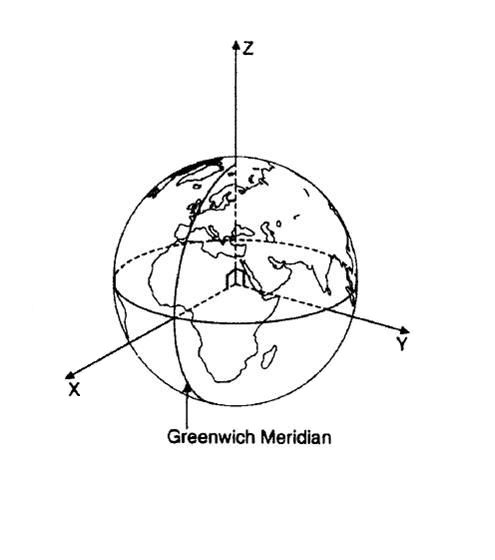
\includegraphics[scale=0.4]{eci_frame.jpg}
\centering
\label{fig:eci_frame}
\caption{ECI frame, Image \cite{larson1992space}}
\end{figure}
\subsubsection{ECEF frame}
This frame also has its origin at the center of the Earth, but the Earth Centered Earth
Fixed frame has its x-axis pointing towards the point where the intersection between the
longitude and latitude have zero value. It can also be described as the intersection between
the Greenwich meridian and the Equator. The frame’s z-axis is pointing along the Earth’s
rotation axis. The y-axis completes the right handed orthogonal system. The ECEF frame
is not an inertial frame, it rotates relative to the ECI frame along the Earth rotation.
\subsubsection{NED frame}
The North East Down frame has its z-axis pointing downwards, perpendicular to the tan-
gent plane of the Earth’s reference ellipsoid. The ellipsoid is mathematically defined and
fitted for approximation of the Earth. The x-axis points towards true north and the y-axis
points East. The NED frame is an inertial frame.
\subsubsection{BODY frame}
This frame is attached to the satellite, and is moving and rotating with it. The origin
coincides with the origin of the NED frame. The axes coincide with the principle axes
of inertia; the x-axis is pointing forwards, the y-axis is pointing to the right side and the
z-axis is pointing downwards through the camera side of the satellite.
\begin{figure}[h]
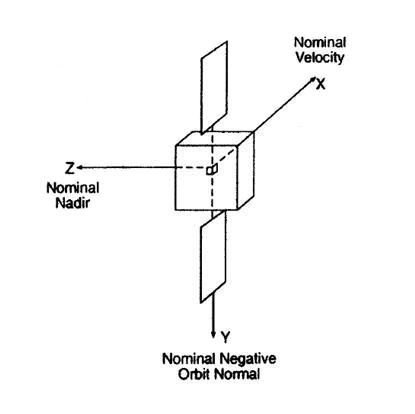
\includegraphics[scale=0.5]{body_frame.jpg}
\centering
\label{fig:body_frame}
\caption{BODY frame, Image \cite{larson1992space}}
\end{figure}
\subsection{Space environment}
\subsection{Attitude representations}
Several representations for describing attitude are available, the most common being Euler
angles. More complicated attitude representations are quaternions. Quaternions are used
for all the estimation methods presented in this thesis. They are singular-free, and are
therefore well suited for attitude determination.
\subsubsection{Euler angles}
\cite{euler1775formulae}
\begin{equation}
\bm{R}_x(\phi) = \begin{bmatrix}
1 & 0 & 0 \\
0 & \cos(\phi) & -sin(\phi) \\
0 & \sin(\phi) & \cos(\phi)
\end{bmatrix}
\end{equation}
\begin{equation}
\bm{R}_y(\theta) = \begin{bmatrix}
\cos(\theta) & 0 & \sin(\theta) \\
0 & 1 & 0 \\
-\sin(\theta) & 0 & \cos(\theta)
\end{bmatrix}
\end{equation}
\begin{equation}
\bm{R}_z(\psi) = \begin{bmatrix}
\cos(\psi) & -\sin(\psi) & 0 \\
\sin(\psi) & \cos(\psi) & 0 \\
0 & 0 & 1
\end{bmatrix}
\end{equation}
\subsubsection{Quaternions}
\cite{hamilton1844lxxviii}\par
\cite{cayley1845xiii}\par
\cite{courant1953methods}\par
\cite{mebius2005matrix}\par
\cite{mathworldconjugate}\par
\cite{shoemake1985animating}\par
\cite{horn1987closed}\par
\begin{equation}
\bm{q} \coloneqq \begin{bmatrix}
q_0 \\
q_1 \\
q_2 \\
q_3
\end{bmatrix}
\end{equation}
\begin{equation}
q_0 = \cos(v/2)
\end{equation}
\begin{equation}
\bm{n} = \frac{\bm{n}}{||\bm{n}||}
\end{equation}
\begin{equation}
\bm{q}_{vec} \coloneqq \begin{bmatrix}
q_1 \\
q_2 \\
q_3
\end{bmatrix}
= [\bm{n}\sin(v/2)]
\end{equation}
\begin{equation}
\bm{q} \coloneqq q_0 + \bm{q}_vec = q_0 + q_1i + q_2j+ q_3k
\end{equation}
\begin{equation}
\bm{Q} = \begin{bmatrix}
q_0 & -q_1 & -q_2 & -q_3 \\
q_1 & q_0 & -q_3 & q_2 \\
q_2 & q_3 & q_0 & -q_1 \\
q_3 & -q_2 & q_1 & q_0
\end{bmatrix}
\end{equation}
\begin{equation}
\bm{q}^* \coloneqq q_0 - \bm{q}_{vec} = q_0 + q_1i + q_2j+ q_3k
\end{equation}
\begin{equation}
\bm{q}^T\bm{q} = 1
\end{equation}
\subsection{Quaternion properties}
\subsubsection{Advantages of quaternions}
\subsubsection{Multiplication of quaternions}
\subsubsection{Quaternions and rotations}
\subsection{Cholesky factorization}
\subsection{Lyapunov analysis}

\newpage
\section{Star-tracker program}
\cite{ju2003overview}\par
Generally star-tracker is divided into three main parts\cite{6187242}:
\begin{itemize}
\item recogiting stars on the image and converting the data into list of star vectors by calculating star centroids;
\item identyfing which star vector represents which real star in catalogue. This is done by comparing star vectors from the image with data in star catalogue, which is generated before space mission;
\item estimating the attitude by calculating the displacement between two frames.
\end{itemize}
\subsection{Centroid - start recognition}
\cite{samaan2002predictive}

\cite{liebe2002accuracy}

Due to limitations of camera there exists necessity of calculating star centroids. Each camera converts image into photo divided by pixels. As it is necessary to have high precision of star coordinates, the pixel accuracy is not enough. Subpixel accuracy is needed. Typically it is done by defocusing the lens of the camera and calculating the lumosity of all pixels around the lightest ones. The idea of how to calculate such centroids is adapted from\cite{6187242}.

If FOV is too small, one star will be considered by program as few stars, and if FOV is too large, few stars placed near each other will be considered as one star. Calculating star centroids is tradeoff between counting few stars as one and counting one star as a few. It seems however that it is worse to count one star as few than few stars as one.

\begin{equation}
x_{start} = x - \frac{a_{ROI} - 1}{2}
\end{equation}
\begin{equation}
y_{start} = y - \frac{a_{ROI} - 1}{2}
\end{equation}
\begin{equation}
x_{end} = x_{start} + a_{ROI}
\end{equation}
\begin{equation}
y_{end} = y_{start} + a_{ROI}
\end{equation}
\begin{subequations}
\begin{equation}
I_{bottom} = \sum_{i=1}^{x_{end}-1} I(i, y_{start})
\end{equation}
\begin{equation}
I_{top} = \sum_{i=2}^{x_{end}} I(i, y_{end})
\end{equation}
\begin{equation}
I_{left} = \sum_{j=1}^{y_{end}-1} I(x_{start}, j)
\end{equation}
\begin{equation}
I_{right} = \sum_{j=2}^{y_{end}} I(x_{start}, j)
\end{equation}
\begin{equation}
I_{border} = \frac{I_{top} + I_{bottom} + I_{left} + I_{right}}{4(a_{ROI} - 1)}
\end{equation}
\end{subequations}
\begin{equation}
\tilde{I}(x,y) = I(x,y) - I_{border}
\end{equation}

\begin{equation}
B = \sum_{i=x_{start}+1}^{x_{end}-1}\sum_{j=y_{start}+1}^{y_{end}-1}\tilde{I}(i,j)
\end{equation}
\begin{equation}
x_{CM} = \sum_{i=x_{start}+1}^{x_{end}-1}\sum_{j=y_{start}+1}^{y_{end}-1}\frac{i \times \tilde{I}(i,j)}{B}
\end{equation}
\begin{equation}
x_{CM} = \sum_{i=x_{start}+1}^{x_{end}-1}\sum_{j=y_{start}+1}^{y_{end}-1}\frac{j \times \tilde{I}(i,j)}{B}
\end{equation}

\begin{equation}
u = \frac{
\begin{bmatrix}
\mu x_{CM} & \mu y_{CM} & f
\end{bmatrix}
^T}
{||
\begin{bmatrix}
\mu x_{CM} & \mu y_{CM} & f
\end{bmatrix}
||}
\end{equation}

\subsection{Star identification}
all \cite{spratling2009survey}\par
Brightness Independent 4-Star Matching Algorithm for Lost-in-Space 3-Axis Attitude Acquisition\cite{dong2006brightness} \par
SP-Search: A New Algorithm for Star Pattern Recognition \cite{mortari1999sp} \par
Star Identification using Neural networks \cite{miri2012star} \cite{lindbladstar} \par
Star pattern recognition using neural networks \cite{li2003star} \par


\subsubsection{Angle Matching}
% https://books.google.pl/books?id=GtzzpUN8VEoC&pg=PA259&lpg=PA259&dq=Gottlieb+Star+Identification+Techniques+1978&source=bl&ots=6_y_cnQUJe&sig=TBkqnYn41hOWcswFdt1a1fghNcc&hl=en&sa=X&ved=0ahUKEwjuiriUuNnOAhWE_iwKHX46AIgQ6AEIIDAA#v=onepage&q=Gottlieb%20Star%20Identification%20Techniques%201978&f=false

\begin{figure}[h]
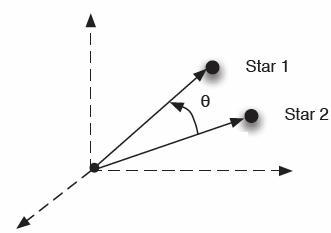
\includegraphics[scale=0.7]{vector_angle_method.jpg}
\centering
\label{fig:angle_matching}
\caption{Vector angle method, Image \cite{gottlieb1978star}?}
\end{figure}

\cite{gottlieb1978star}
\begin{equation}
\theta = \cos^{-1}(\bm{r}_1 \cdot \bm{r}_2)
\end{equation}
\begin{equation}
\bm{b}_i = A\bm{r}_i
\end{equation}
\begin{equation}
\tilde{\bm{b}}_i = A\bm{r}_i + \bm{v}_i, \hspace{0.5cm} \bm{v}_i^TA\bm{r}_i = 0
\end{equation}
\begin{subequations}
\begin{equation}
E\left\{\bm{v}_i\right\} = 0
\end{equation}
\begin{equation}
E\left\{\bm{v}_i\bm{v}_i^T\right\} = \sigma_i^2 [\bm{I} - (A\bm{r}_i)(A\bm{r}_i)^T]
\end{equation}
\end{subequations}
\begin{equation}
\bm{b}_i^T\bm{b}_j = \bm{r}_i^TA^TA\bm{r}_j = \bm{r}_i^T\bm{r}_j
\end{equation}
\begin{subequations}
\begin{align*}
\tilde{\bm{b}}_i = A\bm{r}_i + \bm{v}_i\\
\tilde{\bm{b}}_j = A\bm{r}_j + \bm{v}_j
\end{align*}
\end{subequations}
\begin{equation}
z \equiv \tilde{\bm{b}}_i^T\tilde{\bm{b}}_j = \bm{r}_i^T\bm{r}_j + \bm{r}_i^TA^T\bm{v}_J + \bm{r}_j^TA^T\bm{v}_i + \bm{v}_i^T\bm{v}_j
\end{equation}
\begin{equation}
E\left\{z\right\} = \bm{r}_i^T\bm{r}_j
\end{equation}
\begin{equation}
p \equiv z - E\left\{z\right\} = \bm{r}_i^TA^T\bm{v}_J + \bm{r}_j^TA^T\bm{v}_i + \bm{v}_i^T\bm{v}_j
\end{equation}
\begin{equation}
\begin{split}
\sigma_p^2 \equiv E\left\{p\right\} = \\
\bm{r}_1^TA^TR_2A\bm{r}_1 + \bm{r}_2^TA^TR_aA\bm{r}_2 + Trace(R_1R_2) = \\
Trace(A\bm{r}_1\bm{r}_1^TR_2) + Trace(A\bm{r}_2\bm{r}_2^TR_1) + Trace(R_1R_2)
\end{split}
\end{equation}
\subsubsection{Spherical Triangle Matching}

\begin{figure}[h]
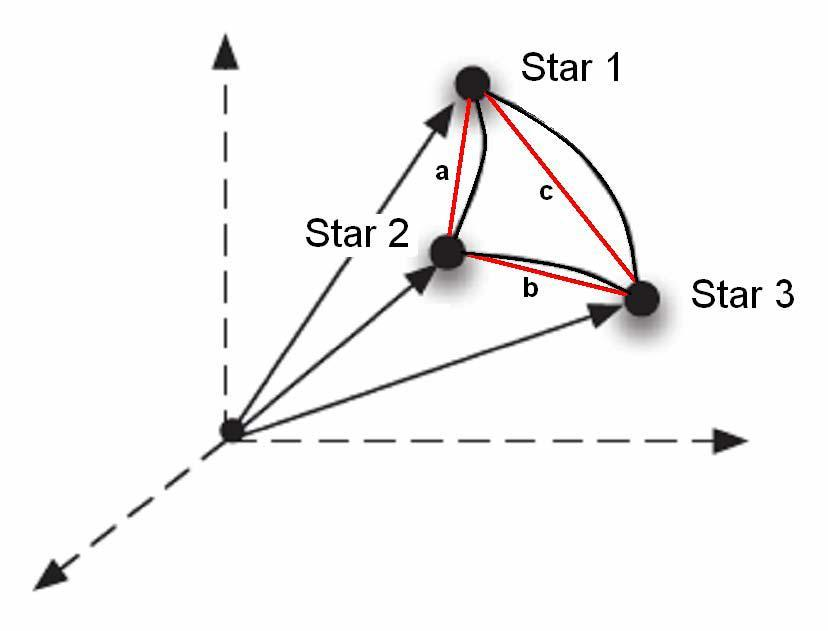
\includegraphics[scale=0.29]{spherical_triangle_method.jpg}
\centering
\label{fig:spherical_triangle_method}
\caption{Spherical Triangle Method, Image \cite{cole2004fast}?}
\end{figure}

\cite{cole2004fast}

\begin{equation}
A = 4\tan^{-1}\sqrt{\tan\frac{s}{2}\tan\frac{s-a}{2}\tan\frac{s-b}{2}\tan\frac{s-c}{2}}
\end{equation}
\begin{subequations}
\begin{align*}
s = \frac{1}{2}(a + b + c) \\
a = \cos^{-1} \bigg(\frac{b_1 \cdot b_2}{|b_1||b_2|}\bigg) \\
b = \cos^{-1} \bigg(\frac{b_2 \cdot b_3}{|b_2||b_3|}\bigg) \\
c = \cos^{-1} \bigg(\frac{b_3 \cdot b_1}{|b_3||b_1|}\bigg) 
\end{align*}
\end{subequations}
\begin{equation}
I_p = \sum\theta^2dA
\end{equation}
\subsubsection{Planar Triangle}

\begin{figure}[h]
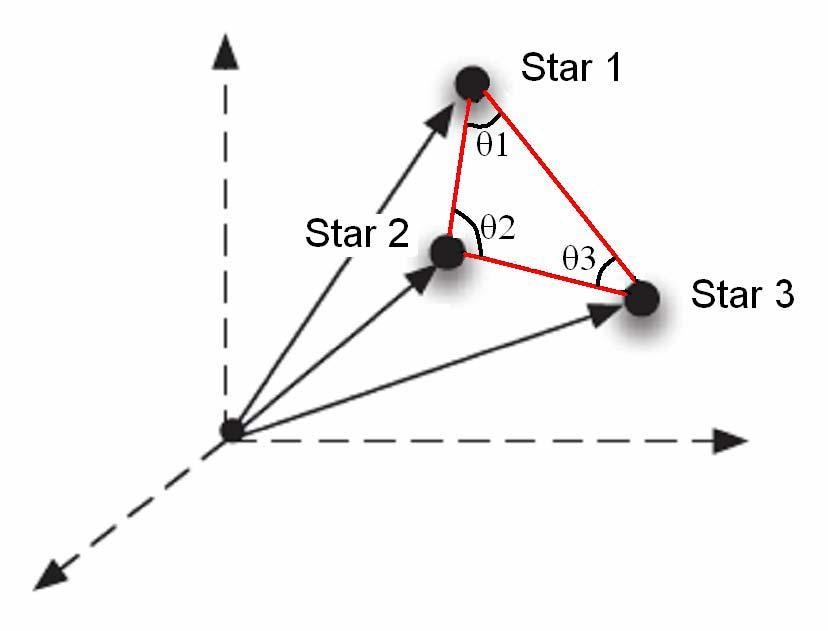
\includegraphics[scale=0.30]{planar_triangle_method.jpg}
\centering
\label{fig:planar_triangle_method}
\caption{Planar Triangle Method, Image \cite{cole2006fast}?}
\end{figure}

\cite{cole2006fast}\par

\begin{subequations}
\begin{equation}
s = \frac{1}{2}(a + b + c)
\end{equation}
\begin{equation}
a = ||\bm{u_p} - \bm{u_q}||
\end{equation}
\begin{equation}
b = ||\bm{u_q} - \bm{u_r}||
\end{equation}
\begin{equation}
c = ||\bm{u_p} - \bm{u_r}||
\end{equation}
\end{subequations}
\begin{equation}
A = \sqrt{s(s-a)(s-b)(s-c)}
\end{equation}
\begin{equation}
J = A\frac{(a^2 + b^2 + c^2)}{36}
\end{equation}

Derivatives
\begin{equation}
H = \begin{bmatrix}
\bm{h}_1^T & \bm{h}_2^T & \bm{h}_3^T
\end{bmatrix}
\end{equation}

\begin{subequations}
\begin{equation}
\bm{h}_1^T \equiv \frac{\delta A}{\delta a}\frac{\delta a}{\delta\bm{b}_1} + \frac{\delta A}{\delta c}\frac{\delta c}{\delta\bm{b}_1}
\end{equation}
\begin{equation}
\bm{h}_2^T \equiv \frac{\delta A}{\delta a}\frac{\delta a}{\delta\bm{b}_2} + \frac{\delta A}{\delta b}\frac{\delta b}{\delta\bm{b}_2}
\end{equation}
\begin{equation}
\bm{h}_3^T \equiv \frac{\delta A}{\delta b}\frac{\delta b}{\delta\bm{b}_3} + \frac{\delta A}{\delta c}\frac{\delta c}{\delta\bm{b}_3} 
\end{equation}
\end{subequations}

\begin{subequations}
\begin{equation}
\frac{\delta A}{\delta a} = \frac{u_1 - u_2 + u_3 + u_4}{4A}
\end{equation}
\begin{equation}
\frac{\delta A}{\delta b} = \frac{u_1 + u_2 - u_3 + u_4}{4A}
\end{equation}
\begin{equation}
\frac{\delta A}{\delta c} = \frac{u_1 + u_2 + u_3 - u_4}{4A}
\end{equation}
\end{subequations}

\begin{subequations}
\begin{equation}
u_1 = (s - a)(s - b)(s - c)
\end{equation}
\begin{equation}
u_2 = s(s - b)(s - c)
\end{equation}
\begin{equation}
u_3 = s(s - a)(s - c)
\end{equation}
\begin{equation}
u_4 = s(s - a)(s - b)
\end{equation}
\end{subequations}

\begin{subequations}
\begin{equation}
\frac{\delta a}{\delta \bm{b}_1} = (\bm{b}_1 - \bm{b}_2)^T /a, \hspace{0.5cm} \frac{\delta a}{\delta \bm{b}_2} = -\frac{\delta a}{\delta \bm{b}_1}
\end{equation}
\begin{equation}
\frac{\delta b}{\delta \bm{b}_2} = (\bm{b}_2 - \bm{b}_3)^T /b, \hspace{0.5cm} \frac{\delta b}{\delta \bm{b}_3} = -\frac{\delta b}{\delta \bm{b}_2}
\end{equation}
\begin{equation}
\frac{\delta c}{\delta \bm{b}_1} = (\bm{b}_1 - \bm{b}_3)^T /c, \hspace{0.5cm} \frac{\delta c}{\delta \bm{b}_3} = -\frac{\delta c}{\delta \bm{b}_1}
\end{equation}
\end{subequations}

\begin{equation}
\sigma_A^2 = HRH^T
\end{equation}

\begin{equation}
R \equiv \begin{bmatrix}
R_1 & 0_{3x3} & 0_{3x3} \\
0_{3x3} & R_2 & 0_{3x3} \\
0_{3x3} & 0_{3x3} & R_3
\end{bmatrix}
\end{equation}

Polar Moment

\begin{equation}
\bar{H} = \begin{bmatrix}
\bar{\bm{h}}_1^T & \bar{\bm{h}}_2^T & \bar{\bm{h}}_3^T
\end{bmatrix}
\end{equation}

\begin{subequations}
\begin{equation}
\bar{\bm{h}}_1^T \equiv \frac{\delta J}{\delta a}\frac{\delta a}{\delta\bm{b}_1} + \frac{\delta J}{\delta c}\frac{\delta c}{\delta\bm{b}_1} + \frac{\delta J}{\delta A}\bm{h}_1^T
\end{equation}
\begin{equation}
\bar{\bm{h}}_2^T \equiv \frac{\delta J}{\delta a}\frac{\delta a}{\delta\bm{b}_2} + \frac{\delta J}{\delta b}\frac{\delta b}{\delta\bm{b}_2} + \frac{\delta J}{\delta A}\bm{h}_2^T
\end{equation}
\begin{equation}
\bar{\bm{h}}_3^T \equiv \frac{\delta J}{\delta b}\frac{\delta b}{\delta\bm{b}_3} + \frac{\delta J}{\delta c}\frac{\delta c}{\delta\bm{b}_3} + \frac{\delta J}{\delta A}\bm{h}_3^T
\end{equation}
\end{subequations}

\begin{subequations}
\begin{equation}
\frac{\delta J}{\delta a} = A a/18, \hspace{0.5cm} \frac{\delta J}{\delta a} = A b/18, \hspace{0.5cm} \frac{\delta J}{\delta a} = A c/18
\end{equation}
\begin{equation}
\frac{\delta J}{\delta A} = (a^2 + b^2 + c^2)/36
\end{equation}
\end{subequations}

\begin{equation}
\sigma_J^2 = \bar{H}R\bar{H}^T
\end{equation}

\subsubsection{Pyramid}

\begin{figure}
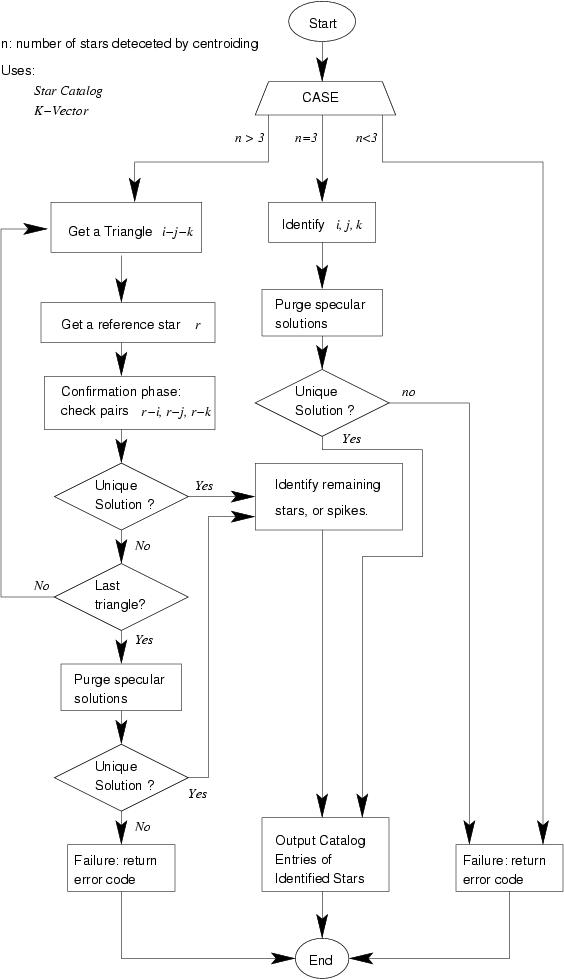
\includegraphics[scale=0.57]{pyramid_method.jpg}
\centering
\label{fig:pyramid_method}
\caption{Pyramid Method Flowchart, Image \cite{mortari2004pyramid}}
\end{figure}

\cite{mortari2004pyramid}\par


\subsubsection{Rate Matching}
\cite{samaan2005recursive}
to be removed?
\subsubsection{Voting}
\cite{kolomenkin2008geometric} \par
\subsubsection{Grid}
%http://dsp.ucsd.edu/~kreutz/Publications/Padgett1997.pdf
\cite{padgett1997grid}
\subsection{Star-catalogue and searching for matching stars}

\subsubsection{Star Catalogue Generation}
\begin{equation}
\bm{u} = \begin{bmatrix}
\cos \alpha \cos \delta \\
\sin \alpha \cos \delta \\
\sin \delta
\end{bmatrix}
\end{equation}
\begin{equation}
m_i \leq m_{max}
\end{equation}
\begin{equation}
m_j \leq m_{max}
\end{equation}
\begin{equation}
\bm{u_a^T u_b} \geq \cos \theta_{FOV}
\end{equation}

\subsubsection{Candidate Matching}
to be removed?
\subsubsection{Result Verification}
to be removed?
\subsubsection{k-vector}
The k-vector database is built a priori for some given working
magnitude threshold and for the star tracker maximum angular aperture. Essentially, the
k-vector table is a structural database of all cataloged star pairs that could possibly fit in the
camera FOV over the whole sky. The star pairs are ordered with increasing interstar angle.
The data stored are the k index, the cosine of the interstar angle, and the master catalog
indices I[k] and J[k] of the kth star pair. The k-vector access logic is invoked in real time
for a minimal set of star pairs in elementary measured star polygons (three for a triangle,
six for a four-star pyramid, etc.); the fact that the vertices between adjacent measured star
pairs share a common cataloged star is the key observation leading to logic for efficiently
identifying the stars by simply comparing the k-vector accessed catalog indices from the
several sets of candidate star pairs (which must contain the common measured pivot star, if
it is in the catalog).
\cite{mortari2013k}\par
\cite{mortari1996fast}\par
\cite{mortari2000k}\par
Trzeba dodać pogrubienia vectorów
\begin{equation}
z(x) = mx + q
\end{equation}
\begin{equation}
m = \frac{y_{max} - y_{min} + \delta\epsilon}{n - 1}
\end{equation}
\begin{equation}
q = y_{min} - m - \delta\epsilon
\end{equation}
\begin{equation}
\epsilon \approx 22.2 \times 10^{-16}
\end{equation}
\begin{equation}
\delta\epsilon = (n - 1)\epsilon
\end{equation}
\begin{equation}
k(i) = j \hspace{0.5cm} where \hspace{0.5cm} s(j) \leq z(i) < s(j + 1)
\end{equation}
or
\begin{equation}
k(i) = j \hspace{0.5cm} \textnormal{where j is the greatest index such} \hspace{0.5cm} s(j) \leq y(I(i)) \hspace{0.5cm} \textnormal{is satisfied.}
\end{equation}
\begin{equation}
j_b = \Big\lfloor\frac{y_a - q}{m}\Big\rfloor \hspace{0.5cm} and \hspace{0.5cm} j_t = \Big\lceil\frac{y_b - q}{m}\Big\rceil
\end{equation}
\begin{equation}
k_{start} = k(j_b) + 1 \hspace{0.5cm} and \hspace{0.5cm} k_{end} = k(j_t)
\end{equation}
\subsection{Attitude Determination}
\cite{jenssen2011comparison}\par
AIM (Attitude estimation using Image Matching)\cite{delabie2012highly}\par
all \cite{hall2003spacecraft} \cite{markley1999estimate}
\subsubsection{The Predictive Attitude Determination Algorithm ?}
\cite{park2006attitude}
\subsubsection{q-method}

\begin{equation}
\bm{s}_b = \bm{R}^{bi}\bm{s}_i \hspace{0.5cm} \bm{m}_b = \bm{R}^{bi}\bm{m}_i
\end{equation}

\begin{equation}
\begin{split}
J &= \frac{1}{2} \sum w_k (\bm{v}_{kb} - \bm{R}^{bi} \bm{v}_{ki})^T (\bm{v}_{kb} - \bm{R}^{bi} \bm{v}_{ki}) \\ 
&= \frac{1}{2} \sum w_k (\bm{v}_{kb}^T\bm{v}_{kb} + \bm{v}_{ki}^T\bm{v}_{ki} + 2\bm{v}_{kb}^T \bm{R}^{bi} \bm{v}_{ki})
\end{split}
\end{equation}


\begin{equation}
J = \sum w_k (1 - \bm{v}_{kb}^T \bm{R}^{bi} \bm{v}_{ki})
\end{equation}

\begin{equation}
g(\bm{R}) = \sum w_k \bm{v}_{kb}^T \bm{R}^{bi} \bm{v}_{ki}
\end{equation}

\begin{equation}
\bm{R} = (q_4^2 - \bm{q}^T\bm{q})1 + 2\bm{qq}^T - 2q_4\bm{q}^{\bm{x}}
\end{equation}

\begin{equation}
\bm{\bar{q}}^T\bm{\bar{q}} = 1
\end{equation}

\begin{equation}
g(\bm{\bar{q}}) = \bm{\bar{q}}^T\bm{K}\bm{\bar{q}}
\end{equation}

\begin{equation}
\bm{K} = \begin{bmatrix}
\bm{S} - \sigma\bm{I} & \bm{Z} \\
\bm{Z}^T & \sigma
\end{bmatrix}
\end{equation}

\begin{equation}
\bm{B} = \sum_{k=1}^Nw_k(\bm{v}_{kb}\bm{v}_{ki}^T)
\end{equation}

\begin{equation}
\bm{S} = \bm{B} + \bm{B}^T
\end{equation}

\begin{equation}
\bm{Z} = \begin{bmatrix}
B_{23} - B_{32} & B_{32} - B_{13} & B_{12} - B_{21}
\end{bmatrix} ^T
\end{equation}

\begin{equation}
\sigma = tr[\bm{B}]
\end{equation}

\begin{equation}
g'(\bm{\bar{q}}) = \bm{\bar{q}}^T\bm{K}\bm{\bar{q}} - \lambda\bm{\bar{q}}^T\bm{\bar{q}}
\end{equation}

\begin{equation}
\bm{K}\bm{\bar{q}} = \lambda\bm{\bar{q}}
\end{equation}

\begin{equation}
g(\bm{\bar{q}}) = \bm{\bar{q}}^T\bm{K}\bm{\bar{q}} = \bm{\bar{q}}^T\lambda\bm{\bar{q}} = \lambda\bm{\bar{q}}^T\bm{\bar{q}} = \lambda
\end{equation}

\subsubsection{Wahba's problem}
\cite{wahba1965least}

\begin{equation}
\sum_j^n ||r_j - Mb_j||
\end{equation}
\subsubsection{QUEST}
improvement to quest implementation \cite{RIS_1} \par
kallman filtering \cite{shuster1990kalman}
\begin{equation}
\begin{split}
J(\bm{q}) = \frac{1}{2}\sum_{j=1}^n\frac{1}{\sigma_j^2}(\bm{b}_j - \bm{R}_b^i(\bm{q})\bm{r}_j)^T(\bm{b}_j - \bm{R}_b^i(\bm{q})\bm{r}_j) = \\
\frac{1}{2}\sum_{j=1}^n\frac{1}{\sigma_j^2}(\bm{b}_j^T\bm{b}_j - 2\bm{b}_j^T\bm{R}_b^i(\bm{q})\bm{r}_j + \bm{r}_j^T\bm{r}_j)
\end{split}
\end{equation}
\begin{equation}
J(\bm{q}) = \sum_{j=1}^n\frac{1}{\sigma_j^2}(1 - \bm{b}_j^T\bm{R}_b^i(\bm{q})\bm{r}_j)
\end{equation}
\subsubsection{TRIAD}
a must
\subsubsection{The Fast Optimal Attitude Matrix}
to be removed?
\subsubsection{DCM (Direction Cosine Matrix)}
\cite{juang2003efficient}
 and

\cite{6187242}
\begin{equation}
\bm{B = \sum_{i=1}^nb_ir_i^T}
\end{equation}
\begin{equation}
\bm{B = USV^T}
\end{equation}
\begin{equation}
\bm{U}_+ = \bm{U}\begin{bmatrix}
1 & 0 & 0 \\
0 & 1 & 0 \\
0 & 0 & det\bm{U}
\end{bmatrix}
\end{equation}
\begin{equation}
\bm{V}_+ = \bm{V}\begin{bmatrix}
1 & 0 & 0 \\
0 & 1 & 0 \\
0 & 0 & det\bm{V}
\end{bmatrix}
\end{equation}
\begin{equation}
\bm{A = U_+V_+^T}
\end{equation}
\newpage
\section{Prototype}
For now the following parts are finished in Python:
\begin{enumerate}
\item Centroiding
\item Planar Triangle Recognition with variations (nearly)
\item Pyramid alg ?
\item k-vector
\item QUEST (not started yet)
\end{enumerate}
Testing\par
\cite{kruijff2003star}
\newpage
\section{Complete program}

\newpage
\section{Testing of star-tracker}
\cite{RIS_0}

\newpage
\bibliographystyle{ieeetr}
\bibliography{bibfile}




\newpage

\listoftables

\newpage

\listoffigures

\newpage


Robot Learning Darmstadt
Problems with Euler Angles:
Not Unique: Many angles result in the same rotation
Hard to quantify differences between two Euler Angles
Unit-Quaternion
Solves the problems of singularities with the Euler Angles
Easier to compute differences of orientations
Important if we want to control the orientation of the end-effector
See Siciliano or Spong Textbook!

%https://en.wikipedia.org/wiki/Apparent_magnitude

Polar moment

\end{document}
